\documentclass[pdftex,11pt]{article}

%\usepackage[scaled=0.94]{helvet}
%\renewcommand{\familydefault}{\sfdefault}

\usepackage{fullpage,amssymb,amsmath}
\usepackage{graphicx}
\usepackage{natbib}
\usepackage{times}
\usepackage[T1]{fontenc}
\usepackage{color}
\usepackage[pdftex,pdfborderstyle={/S/U/W 1},hyperfootnotes=false,colorlinks]{hyperref}
\usepackage[pdftex,hyperfootnotes=false]{hyperref}
\hypersetup{pageanchor=false}
\usepackage[usenames,dvipsnames]{xcolor}
\hypersetup{citecolor=MidnightBlue}
\hypersetup{linkcolor=Black}
\hypersetup{urlcolor=MidnightBlue}
\usepackage{wrapfig}
\usepackage{bm}
\usepackage{amsmath}
\usepackage{stmaryrd}
\usepackage{multicol,multirow}
\usepackage{colortbl}

\SetSymbolFont{stmry}{bold}{U}{stmry}{m}{n}

%\addtolength{\textheight}{12pt}
%\addtolength{\topsep}{-5pt}
\addtolength{\textheight}{4pt}
\addtolength{\topsep}{-2pt}
\let\hat\widehat
\let\tilde\widetilde
\renewcommand{\P}{\mbox{$\mathbb{P}$}}
\newcommand{\reals}{\mbox{$\mathbb{R}$}}
\newcommand{\E}{\mbox{$\mathbb{E}$}}
\newcommand{\V}{\mbox{$\mathbb{V}$}}
%\newcommand{\mbx}{\mbox{\boldmath$x$\unboldmath}}
\newcommand{\mbx}{\boldsymbol{x}}
\newcommand{\g}{\,\vert\,}
\long\def\ignore#1{}
\def\given{\,|\,}
\def\LL{h_0}
\newenvironment{proposedwork}{\vskip10pt\setcounter{proposal}{0}}{\vskip10pt}
\def\task#1{\vskip10pt\stepcounter{proposal}\noindent
   {\bf \Alph{proposal}. #1.}\enspace}

\bibpunct{(}{)}{;}{a}{,}{,}
\bibliographystyle{ims}

\newcounter{proposal}
\newcounter{project}
\newcounter{subproposal}
\newcounter{subsubproposal}

\def\msection#1{\vskip30pt\stepcounter{proposal}\setcounter{subproposal}{0}\noindent
   {\bf\Large \arabic{proposal}.\enspace #1}\vskip8pt\noindent}
\def\msubsection#1{\vskip10pt\stepcounter{subproposal}\noindent
   {\bf\large \arabic{proposal}.\arabic{subproposal}.\enspace #1}\enspace\vskip5pt}
\def\msubsubsection#1{\vskip10pt\stepcounter{subsubproposal}\noindent
   {\bf\normalsize \arabic{proposal}.\arabic{subproposal}.\arabic{subsubproposal}\enspace #1}\enspace\vskip5pt}
\def\meme#1{\vskip5pt\noindent {\it\bfseries #1.}\enspace}
\def\background#1{\vskip5pt\noindent {\it\bfseries Background and
    Preliminary Results.}\enspace\setcounter{project}{0}}
\def\project#1{\vskip5pt\noindent {\it\bfseries Proposed Research
    \stepcounter{project}\Alph{project}:  #1.}\enspace}
\def\F{\mathcal{F}}
\let\epsilon\varepsilon
\def\biobackground#1{\vskip5pt\noindent {\it\bfseries Neuroscience
Background.}\enspace\setcounter{project}{0}}
\def\statbackground#1{\vskip5pt\noindent {\it\bfseries Computation and
Inference Background.}\enspace\setcounter{project}{0}}

\renewcommand{\baselinestretch}{0.985}

\begin{document}

%-----------------------------------------------------

\thispagestyle{empty}

\begin{center}
\ 
\vskip-30pt
{{\Large\bf  TRIPODS+X:RES: Investigations at the Interface of \\[5pt]
Data Science and Neuroscience
}}\\[10pt]
{\it Project Summary}
\vskip20pt
\end{center}


\newcounter{aim}
\def\aim#1{\vskip5pt\noindent {\stepcounter{aim}\it\bfseries Objective
    \arabic{aim}:\;\;#1.}\enspace}
\let\objective\aim

The research in this proposal explores the interface between
data science and neuroscience. The overarching theme is to develop
a two-way channel between these fields. 
In one direction, we will investigate how computational
principles from data science can be leveraged to understand recent empirical
findings and advance theory at different levels of neuroscience, 
including cellular measurements in fruit flies and 
whole-brain functional imaging in humans. In the
reverse direction, the project will view the processes and mechanisms
of vision and cognition underlying these findings as a source for
new statistical and mathematical frameworks for data analysis. The research
will focus on four interrelated objectives:


\objective{Distributed processing}
Recent work in machine learning has studied the effect of
communication constraints and parallelization in distributed
estimation. There is a close analogy to vision, where any given input
is sensed by multiple parts of the retina, from which an accurate percept
needs to be constructed. The project will consider different models
for distributed processing, motivated by visual learning and perception in
lower-level organisms. 


\objective{Data representation}
The brain stores the same information in several different ways, each
emphasizing different dimensions of the input. 
%In visual cortex, two
%inputs with similar visual features will be stored together. In
%temporal and frontal cortex, two inputs with the same conceptual or
%semantic meaning/function will be stored together. In the hippocampus, these kinds of
%sensory or semantic overlap are discounted by orthogonalizing similar
%inputs encountered at different times.
Inspired by current understanding of representation
of information in different regions of the cortex, the project will
investigate how parallel lossy representations of the same inputs
along different dimensions can be used for statistically and computationally efficient learning 
algorithms.  In the other direction, we will investigate how embedding
algorithms from machine learning might be used as mechanisms for
processing massive cellular and brain imaging data.

\objective{Attentional filtering} The project will develop
attention-based models in statistical learning, based on the use
of lower-dimensional traces or curves through a high-dimensional
input space. Attention curves have analogues in human cognition, where
input dimensions are processed based on their inherent salience and
relevance to a person's goals. The project will explore mathematical,
computational and empirical models of attention. Experiments will
focus on a public dataset of subjects watching episodes of Sherlock
while being scanned with fMRI, using a frame-by-frame annotation of
several dimensions of the movie as the basis for attention-based models.


\objective{Memory capacity} Evidence from studies of human behavior
suggests that people store information about objects and events in
long-term memory with incredible detail. How is this possible?  
We will consider cognitive studies and
a current understanding of possible memory architectures in natural systems
in order to inform approaches for reducing and sharing memory in
artificial learning algorithms. A framework will be developed for
establishing lower bounds on the risk of machine learning algorithms under
memory constraints. Insights from this mathematical theory will be
considered in the context of memory of complex organisms.



\vskip8pt

\noindent 
The {\it\bfseries intellectual merit} of the proposed research
includes the transfer of ideas between data science and neuroscience,
with the goal of advancing knowledge in both domains.
The {\it\bfseries broader impact} of the research includes development of software that
implements the advanced data science and machine learning algorithms,
the development of labs for an undergraduate course 
in data science with examples drawn from neuroscience, and a series
of workshops hosted at Yale and Brown Universities that expand
the scope of the original TRIPODS effort at Brown.


\newpage


\setcounter{page}{1}
\begin{center}
\ 
\vskip-30pt
{{\Large\bf  TRIPODS+X:RES: Investigations at the Interface of \\[5pt]
Data Science and Neuroscience
}}\\[10pt]
{\it Project Description}
\end{center}


%-----------------------------------------------------
\def\obj#1{\vskip5pt\noindent {\it\bfseries #1.}\enspace}

\msection{Introduction}

This proposal brings together an interdisciplinary team, spanning
mathematics, statistics, computer science, psychology and biology,
to study an interconnected set of objectives at the 
interface between neuroscience and data science. The underlying theme is to develop
a two-way channel between data science and cellular and cognitive
neuroscience. In one direction, we will investigate how computational
principles of data science can be used to understand recent empirical
findings in neuroscience, associated with measurements at the cellular
level in fruit flies, and brain imaging studies in humans. In the
reverse direction, the project will view the processes and mechanisms
of vision and cognition underlying these findings as a source for
new mathematical frameworks for data analysis.  

The research will focus on four interrelated objectives:
distributed processing, data representation, attentional filtering, 
and memory capacity. For each objective, a series of investigations
are proposed that bring together current research
frontiers in neuroscience, statistics, machine learning, and
computation.


\obj{Distributed processing}
The project will consider different models
for distributed processing, motivated by learning and perception in
both lower-level organisms (visual processing in fruit flies) and
higher-level cognition (visual cognition in humans). 


\obj{Data representation}
Inspired by current understanding of representation of information in
different regions of the cortex, the project will investigate how
parallel lossy representations of the same inputs along different
dimensions can be used for statistically and computationally efficient
learning algorithms.  In the other direction, we will investigate how
recent developments in machine learning might be used as mechanisms
for processing massive cellular and brain imaging data.

\obj{Attentional filtering} The project will explore mathematical,
computational and empirical models of attention. One set of analyses will
focus on a public dataset of subjects watching episodes of Sherlock
while being scanned with fMRI, using a frame-by-frame annotation of
several dimensions of the movie as the basis for attention-based models.
Mathematical and statistical models of attention will be developed
as a framework for combating the ``curse of dimensionality''
in complex data.

\obj{Memory capacity} 
We will consider cognitive studies and
a current understanding of possible memory architectures in natural systems
in order to inform approaches for reducing and sharing memory in
artificial learning algorithms. A framework will be developed for
establishing lower bounds on the risk of machine learning algorithms under
memory constraints. A new framework for memory based on generative models
will be studied.

The project is motivated by the transfer of ideas between data science and neuroscience,
to advance knowledge in both domains. It is organized as a component
of the NSF TRIPODS activity at Brown University. Cross-disciplinary
training of graduate students will be a key component of the
activity. In addition, labs for a new undergraduate data science
course at Yale will introduce a neuroscience component that is tied to
the project. Two workshops will be held during the course of the
project. At the end of 



\msection{Distributed Processing (Objective 1)}
\label{sec:aim1}

Recent work in machine learning has studied the effect of
communication constraints and parallelization in distributed
estimation. There is a close parallel in vision, where any given input
is sensed by multiple parts of the retina and an accurate percept
needs to be constructed.


\biobackground{}
Animals use visual cues to guide behavior, from navigation to
foraging and courtship. The perception of these cues is an
inference problem \citep{knill:96}. In this problem, the
animal obtains light intensities from an array of
photoreceptors focused on different points in space. The animal must
combine these signals to infer
and respond to the true state of the world, across several
parallel dimensions of inference. For instance, one dimension of
inference may be the global motion of the visual scene, while
another may be the existence of a predator in the
scene. Neuronal circuits in the visual system perform this
inference task, at lower levels (is there an edge at this location
and angle?) and higher levels (is that object a predator?)
\citep{simoncelli:01}. The processing of 
visual neurons and circuits has been studied in depth, but it is
often unknown how these operational descriptions relate to the
inferences that guide behavior. In particular, these inferences
require integrating distributed retinal information over space and
time, but we do not know how this integration relates to the
statistics of the natural world, to channels of information flow
in circuits, or to noise or incomplete information about the world.

\setlength{\columnsep}{20pt}
\begin{wrapfigure}{R}{0.45\textwidth}
\centering
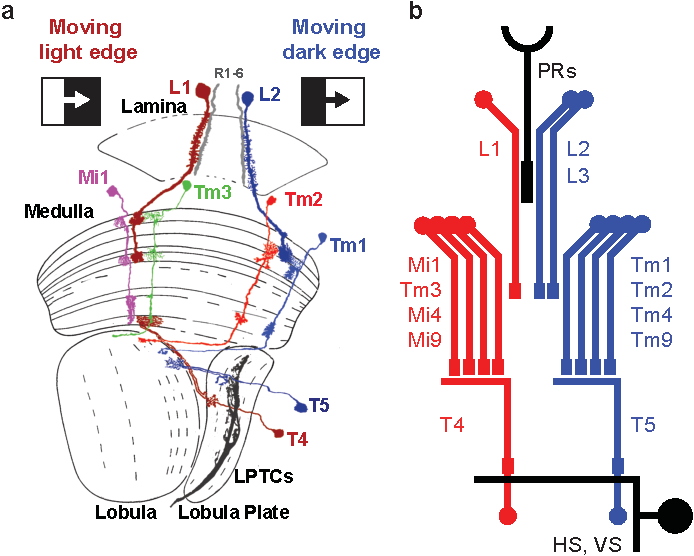
\includegraphics[width=.44\textwidth]{figs/flysetup}
\caption{\small Motion circuits in the fly. (a) Light is detected at the
retina (top), and information is processed
down through different neuropils. Each of the highlighted
neurons is required for motion detection. One circuit 
detects light edges moving over dark backgrounds and another 
detects dark edges over light backgrounds. (b) Cartoon of
neurons known to be involved in motion detection in the light edge
(red) and dark edge (blue) pathways. 
There are four T4s and four T5s, selective for each
of the four cardinal directions across the retina. This circuit repeats at all
points in space.}
    \label{fig:setup}
    \vskip2pt
\end{wrapfigure}

The fruit fly \textit{Drosophila} has several advantages for studying the
distributed visual processing that guides perception and
behavior. First, there is a powerful genetic toolbox in fruit flies
that allows researchers to genetically define, manipulate, and monitor
specific classes of neurons \citep{luo:08}. These manipulations
allow specific neurons to be causally connected to
behaviors. Second, the fly has a wealth of visual behaviors,
including regulation of turning and speed, escape, and
courtship \citep{card:08,silies:14,spieth:74}.
Third, the field has identified neuron types that
appear to be making the inferences described above, including for: 
local motion direction and speed \citep{Maisak:13};
wide-field motion such as rotational
self-motion of the fly about various axes \citep{joesch:08};
looming (approaching) 
dots \citep{devries:12,klapoetke:17}; and 
moving dots \citep{keles:17}. In each case, we
can silence the neurons and observe behavioral deficits. We can also
record activity in these individual neurons and measure their
response properties with well-controlled visual stimuli
\citep{salazar:16}. Thus, these neuron classes act as
handles for understanding how visual inferences are made, and how
neurons extract specific visual features from a spatiotemporally
distributed set of inputs.


\statbackground{}
Statistical theory studies the difficulty of estimation under
various models, and attempts to find optimal estimation
procedures. Such studies usually assume that all of the collected
data are available to construct the estimators. Recent research
has begun to study the problem of statistical estimation in distributed settings, 
as the data can be collected or
stored on multiple machines at different locations. In order to obtain an estimate of some
statistical functional, information needs to be gathered and
aggregated from the multiple locations to form the final
estimate. However, the communication between machines may be
limited. In such a setting, it is important to understand how the
statistical risk of estimation degrades as the communication budget
becomes more constrained.

The so-called CEO problem, first studied in the EE 
community in the context of rate-distortion theory, treats a
similar distributed estimation problem \citep{berger1996ceo,
  viswanathan1997quadratic}. Several later studies
focused on more specific statistical tasks, including mean
estimation, regression, principal eigenspace estimation, and discrete
density estimation \citep{zhang2013information, shamir2014fundamental,
  battey2015distributed, braverman2016communication,
  diakonikolas2017communication, fan2017distributed,
  lee2017communication, shang2017computational}. Most of this 
research treats parametric and discrete models, where the
parameter of interest has finite dimension.  In a nonparametric
setting, the effective dimension of the problem typically grows with
the sample size, and these results no longer apply.
Other results have been obtained on these problems in the normal means
model of nonparametric estimation, which arises naturally when representing an estimator in terms of an
orthogonal
basis \citep{johnstone2002function,tsybakov:2008}.  One
result gives a sharp constrained minimax analysis of nonparametric
regression under quantization constraints \citep{Zhu:18}; another
characterizes lower bounds and achievability for distributed
nonparametric regression \citep{Zhu:18b}. Similar results have been obtained 
using wavelets and Besov spaces \citep{szabo18}.


\project{Parallel channels for local motion detection}
The fly's eye is arranged in a hexagonal lattice of repeated circuit
motifs, with each column of circuitry representing one retinotopic
point in visual space. Each eye consists of an array of ~800 of
these pixels, which together cover approximately one half of visual
space. Two classes of local motion detection cells exist in every
column: T4 cells detect light edges moving across
dark backgrounds and T5 cells detect dark edges moving across
light backgrounds. There are 4 of each class, one for each cardinal
direction, for a total of 8 parallel channels at each point in space
representing motion in two dimensions. Why is the system organized
this way? How are naturalistic motion signals distributed over the 8
channels, and what encoding or decoding advantages does this serve?
Under what conditions are the channels redundant? How would an optimal
observer partition signals among these parallel channels? Could a data-driven 
approach predict or give insight into this encoding scheme?
One approach to begin studying these questions will be to adapt
the classical framework of sparse coding \citep{Olshausen:Field:96}
in a way that represents the neurobiology of the fly's visual system.

\project{Detecting motion flow fields}
When an animal moves or rotates, its
self-motion generates flow fields across its retina. These flow fields
can be used as feedback to control orientation or speed.
In \textit{Drosophila}, some neurons downstream of local motion
detectors have large receptive fields that integrate motion signals
over the retina. They appear selective for specific flow
fields, which correspond to those created by the rotation of
the fly about different axes. These neural signals have been proposed
to be linear filters, matching their weighting for local motion to
specific optical flow fields (``matched filters''). However, it is not
clear whether a linear weighting of local motion estimates is
the best estimate of each field, or whether more complex dendritic
computations could improve encoding. In particular, it is not clear
how these neurons optimally integrate motion signals in the
presence of occlusions or differential velocity fields 
caused by fly translation through space. We will investigate these
issues using methods based on hierarchical sparse coding 
\citep{Yu:2011} and related computational methods for
low-rank decomposition.


\setlength{\columnsep}{10pt}
\begin{wrapfigure}{l}{0.45\textwidth}
\vskip-10pt
\centering
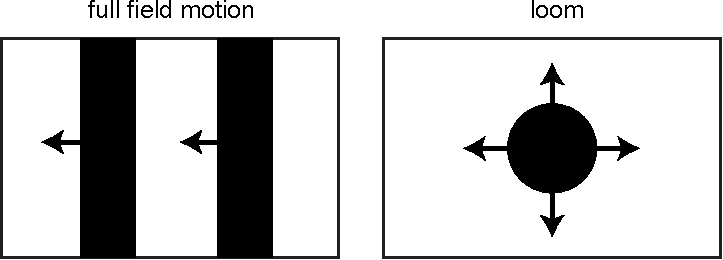
\includegraphics[width=.44\textwidth]{figs/loom}
\caption{\small Global motion and loom generate similar local
motion signals, which must be integrated over space
to distinguish the two stimulus types.}
    \label{fig:loom}
\vskip-20pt
\end{wrapfigure}

\project{Detecting looming stimuli}
Looming stimuli are created by objects as they approach the observer:
the object becomes larger, and if on a collision course,
opposite edges of the object will move in opposite directions on the
retina. Thus, detecting loom requires integrating information over
space, as any local motion detector cannot know if local motion is due
to a looming object or is just wide-field motion. Two neuron types in
\textit{Drosophila} have recently been described as loom detectors,
responding selectively to objects that grow larger in their receptive
fields. The receptive fields of these cells to local motion have been
characterized, but the relationship between these receptive fields,
the nonlinear computations of these neurons, and the statistics of
natural loom stimuli remain unclear. This is partly due to the
absence of natural statistics on loom stimuli. These loom detectors 
may also use features beyond motion to
detect approaching objects. For instance, a detector might integrate
motion signals with light intensity information, since light intensity
is correlated with distance. One might also ask whether the
motion-detecting neurons upstream of the loom-sensitive neurons could
convey information about stimulus features beyond motion
direction and speed. We will abstract loom detection as a statistical
testing problem, building on work such
as \citep{castro:05}.%,huo:06,hc:04}. 
Specifically, for a given object
geometry such as a disk, we will study minimax rates for loom
detection, in terms of the noise level and sparsity of the number of
boundary neuron measurements required. Fast hierarchical algorithms
to achieve the minimax rates will be studied.




\let\tilde\widetilde
\def\SS{{\mathbb S}}
\def\X{{\mathbb X}}
%\def\bb{\mbox{\boldmath$b$}}
\def\bb{b}
\def\noisesd{\sigma}
\def\C{{\mathcal C}}
\def\A{{\mathcal A}}
\def\bigbracket#1#2#3{
\left[ 
\mbox{\begin{minipage}{#1}{
\vskip#2
#3
\vskip#2
\mbox{\ }
}\end{minipage}}
\right]
}

\msection{Data Representation (Objective 2)}
\label{sec:aim2}

The brain persistently stores the same information in several
different ways across regions, each emphasizing different dimensions
of the input. In doing so, different features become readily
accessible to the computations implemented in these regions. More
generally, by representing information in different ways, similar
learning rules are able to automatically aggregate experience along
different dimensions and thereby extract different and complementary
knowledge. This can be contrasted with machine learning, both by the
simple fact that data are stored on disk in one format and that
finding relevant dimensions is often the output of the learning
algorithm rather a natural consequence of how the input is structured.
We will develop algorithms for machine representation of data that are
informed by our understanding of how the brain represents information
in different systems and leverage developments in embedding algorithms
in machine learning for advanced processing of fMRI and cellular
recordings and the information they contain.

\biobackground{} Multiple brain systems represent inputs from the
world and store this information in different memory registers.
Although these representations are sometimes redundant (e.g., across
hemispheres in the same brain system), they often emphasize different
aspects of the input that are extracted via different neural pathways
or as a result of transformations across brain regions. In visual
cortex, for example, different inputs with similar appearance (e.g.,
the faces of siblings, the Grand Canyon from different vistas, bananas
in a grocery store, etc.) will be stored together. In frontotemporal
cortex, different inputs with the same conceptual, semantic, or
functional meaning will be stored together despite differences in
appearance (e.g., pieces of clothing, cooking utensils, animals in the
ocean, etc.). In the ventral striatum and orbitofrontal cortex,
different inputs with the same reward value will be represented
similarly irrespective of appearance or meaning (although subjective,
e.g., a favorite t-shirt and a nostalgic meal, an art show and a music
performance). Finally, in the hippocampus, overlap in appearance,
meaning, and reward can be discounted in favor of representing inputs
that co-occur over space or time together (e.g., a sequence of
landmarks on a commute, the people in a social group, events on a
memorable date, etc.). There are other dimensions that organize or
dominate the representations in other brain systems, such as emotion,
modality, tasks, and motor actions. However, here we will focus on
visual cortex and the hippocampus, two brain systems with mature
theories that address the nature of their representations.

After passing from the retina and through subcortical structures, the
human visual system is a hierarchical set of cortical brain areas
starting from the first visual area (V1) in the calcarine sulcus of
the occipital lobe~\citep{Felleman:1991}. There are four primary
organizing principles from there. First, the visual areas in each
hemisphere receive input from the space contralateral to where the
eyes are fixated (i.e., retinotopic), with the input from a given side
of space projecting to both eyes which converge in ocular dominance
columns in V1. Second, the areas are arrayed into two
streams~\citep{Mishkin:1983,Goodale:1992}: the ventral stream passing
on the inferior surface into the temporal lobe with areas coding for
the contralateral upper quadrant (V1-V3) and then the contralateral
hemifield (V4 and beyond) involved in recognizing the identity of
objects~\citep{Arcaro:2009}; the dorsal stream passing on the superior
surface into the parietal then frontal lobes with areas coding for the
contralateral lower quadrant (V1-V3) and hemifield (V3a and beyond)
involved in processing information about object location and
action~\citep{Konen:2008}. Third, the visual areas in each stream
represent stimulus dimensions of increasing complexity: for example,
from edges in V1, to color and texture in V4, to shape in ventral
occipital, to object identity and category in inferior temporal (IT)
cortex~\citep{Grill-Spector:2003,Rousselet:2004}. Finally, paired with
this increasing complexity is greater flexibility or ``tolerance'' to
variation in more basic features, both in terms of neurons in higher
areas having larger areas of space (i.e., receptive fields) over which
they respond and in terms of invariance of neural representations, in
IT for example, to size, position, viewpoint, etc.~\citep{Rust:2010}.
The properties parallel those of deep convolutional neural networks
for object and scene recognition~\citep{Kriegeskorte:2015}, and in
fact optimizing the architecture of a deep net for object
recognition, without consideration of brain data, naturally
results in a model that predicts neuronal responses in visual
cortex~\citep{Yamins:2016}. The visual system is thus one of the best
understood neurobiological systems and also the one that has had the
greatest impact to date on machine learning.

Most models of ventral visual processing treat IT as the top of
the hierarchy. However, IT is heavily interconnected with
the next most anterior areas, perirhinal cortex (PRC) and
parahippocampal cortex (PHC), which show selectivity for
objects and scenes,
respectively~\citep{Barense:2010,Davachi:2006,Ranganath:2012}. The PRC
and PHC project to the entorhinal cortex (ERC). The ERC in turn
provides input to the hippocampus, which is critical for storing
long-term memories~\citep{Squire:1992}. Within the hippocampus, there
are four key subfields: dentate gyrus (DG), CA3, CA1, and
subiculum~\citep{Deng:2010,Shohamy:2013}. They are
connected to form two pathways: the trisynaptic pathway (TSP) from ERC
to DG, CA3, and CA1; and the monosynaptic pathway (MSP) from ERC to
CA1~\citep{Schapiro:2017}. The hippocampus also has two sources of
recurrence that allow it to bridge over time: locally within CA3 and
as a result of CA1 output to ERC that re-enters as
input~\citep{Kumaran:2016}. The function of the TSP circuit is to
memorize specific input patterns from ERC, supporting ``episodic''
memory for individual moments in space and time (e.g., where I parked
my car this morning). This poses two computational challenges: the
patterns need to be learned ``one-shot'' in that we never experience
the exact same episode twice, and it is critical to avoid interference
from related memories (e.g., where I parked by car yesterday). The TSP
solves these challenges with \textit{pattern
separation}~\citep{Leutgeb:2007,Yassa:2011,Rolls:2016}: large capacity,
strong inhibition, and partial connectivity in DG and then CA3 lead to
sparse, orthogonal representations of even highly overlapping ERC
input patterns that share sensory features (e.g., tend to park in
the same neighborhood, at the same time of day, in the same vehicle,
etc.). The resulting memories are complex, unfurling over space and
time with input from different modalities, and these different
components are linked via the auto-associative connections in
CA3~\citep{Wallenstein:1998}. By discounting feature overlap across
episodes and binding even arbitrary features within episodes, such
spatiotemporal co-occurrence dominates hippocampal representation, allowing for recall of individual experiences.
Whereas theoretical models of the hippocampus from the connectionist
tradition have been around a long time and employ multi-layer
networks~\citep{McClelland:1995,Norman:2003}, the computational
properties of the hippocampus (e.g., pattern separation, different
learning rates, bridging over time, relational binding, etc.) have not
yet entered the mainstream of machine learning.

\setlength{\columnsep}{20pt}
\begin{wrapfigure}{R}{0.45\textwidth}
\centering
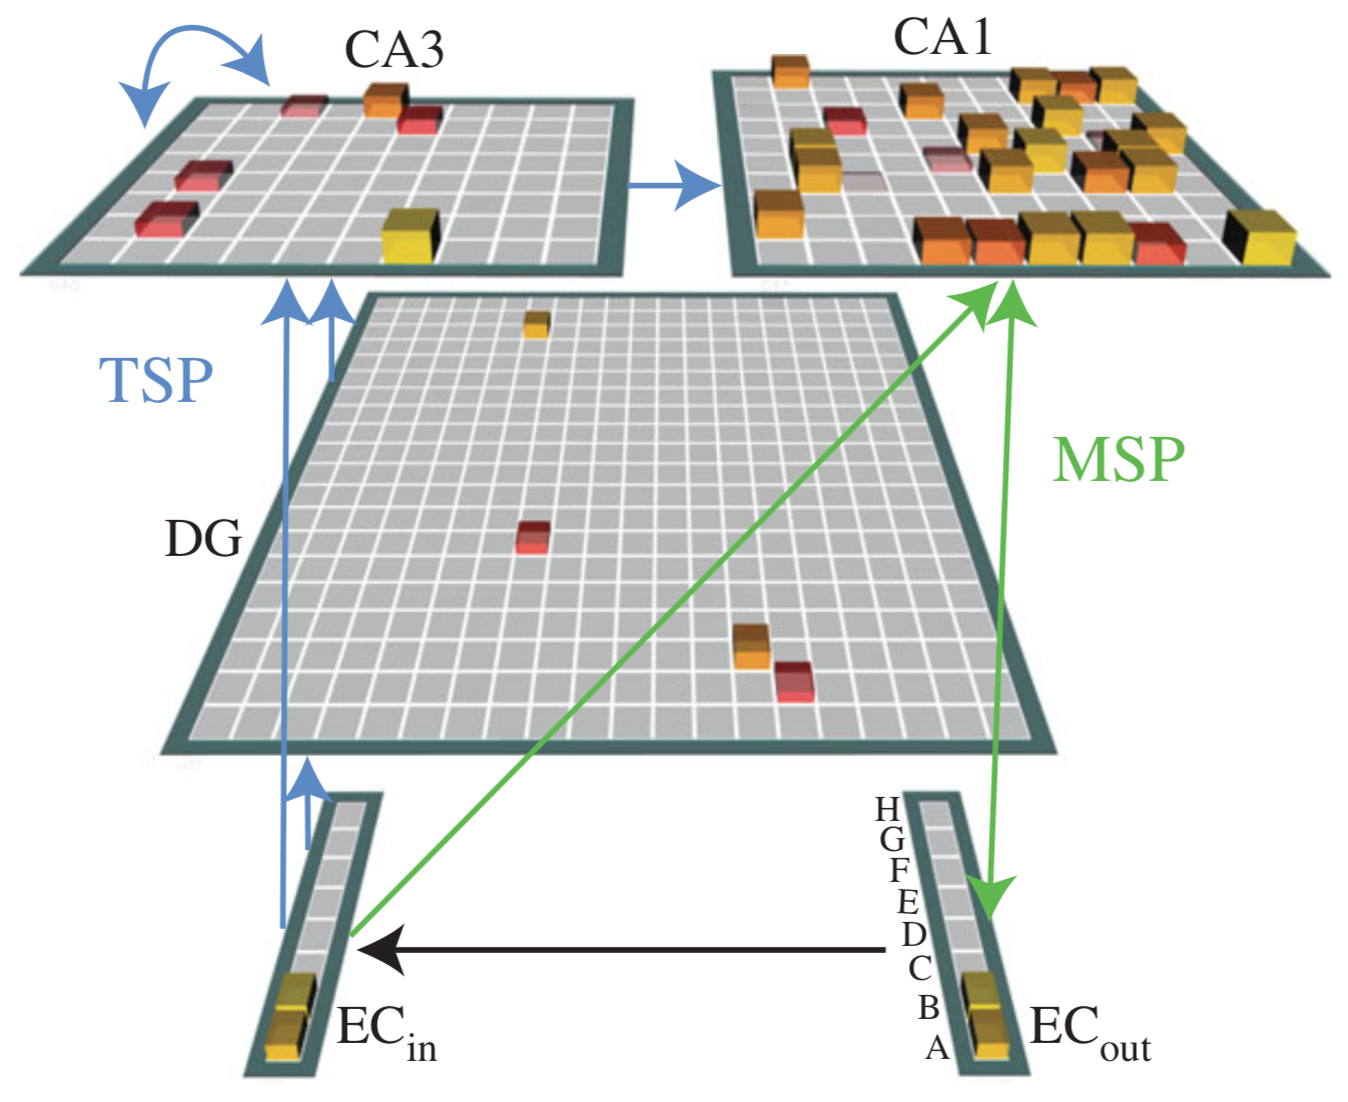
\includegraphics[width=.44\textwidth]{figs/hipp-model}
\caption{\small Biologically plausible neural network model of the
hippocampus. The network is trained to reproduce the pattern of
activity in the input (EC\textsubscript{in}) on the output
(EC\textsubscript{out}). Three hidden layers (DG, CA3, and CA1) learn
representations to support this mapping, with activity flow governed
by projections indicated by the arrows. The TSP, in blue
arrows, supports encoding into episodic memory via pattern separation
in DG and CA3 and retrieval via pattern completion within CA3. The
MSP, in green arrows, supports statistical learning of
regularities across episodes. The height/yellowness of a unit both
index its activity level. From ~\citet{Schapiro:2017}.}
    \label{fig:hipp}
    \vskip2pt
\end{wrapfigure}

\statbackground{}
Data representation algorithms are an important ingredient in contemporary
machine learning methodology. A particular type, called embeddings, are used to represent
categorical data---for example words in a natural language text---as
dense, high dimensional ($d\approx 500$) vectors in Euclidean space \citep{Mikolov:2013}.
Embedding algorithms give representations that are well suited for downstream
algorithms. Sometimes they are learned in the first layer of
a deep neural network ~\citep{Bengio:2003}.  

Embeddings can be useful for many data types. For example, the popular
music entertainment site Spotify constructs embeddings of songs from
millions of user playlists, and uses these as the basis for
recommending new songs.  (``If you liked song $x\in\reals^{500}$,
perhaps you'll like the nearby song $x'\in\reals^{500}$.'')  This
machine learning based system eclipsed Pandora, which was based on a
hand-constructed representation, the ``music genome.'' Yet current
embedding algorithms such as the popular \texttt{word2vec} algorithm
are based on little more than a low-rank approximation (PCA) of simple
co-occurrence statistics.

Embeddings algorithms become more flexible when they are based
on statistical models, for instance using exponential family
models \citep{Rudolph:2016b,spherical}.
Consider a corpus of language $\mbx = \{x_1, \ldots, x_n\}$, where
each $x_i$ is a word from a vocabulary of terms. An exponential family
embedding has three components: (a) a notion of context for
each data point, e.g., a window of observed words around each word (b)
a form of the conditional distribution, e.g., for text a
categorical distribution over $V$ items is appropriate and (c) an
embedding structure that describes how parameters are shared
across data, e.g., for text one may assume that each term (such as
``walnut'' or ``bicycle'') shares the same representations wherever it
appears in the collection.
An exponential family embedding
posits two $d$-dimensional latent representations for each term $v$,
one is the embedding vector $\rho_v$ and the other is the
context vector $\alpha_v$, where $d$ is a hyperparameter.  The
model asserts that each observation is drawn from a conditional
distribution given its context. 
Exponential family embeddings generalize many existing methods for
learning distributed representations, including 
many variants of word2vec~\citep{Mikolov:2013}.  


\setlength{\columnsep}{20pt}
\begin{wrapfigure}{R}{0.45\textwidth}
\centering
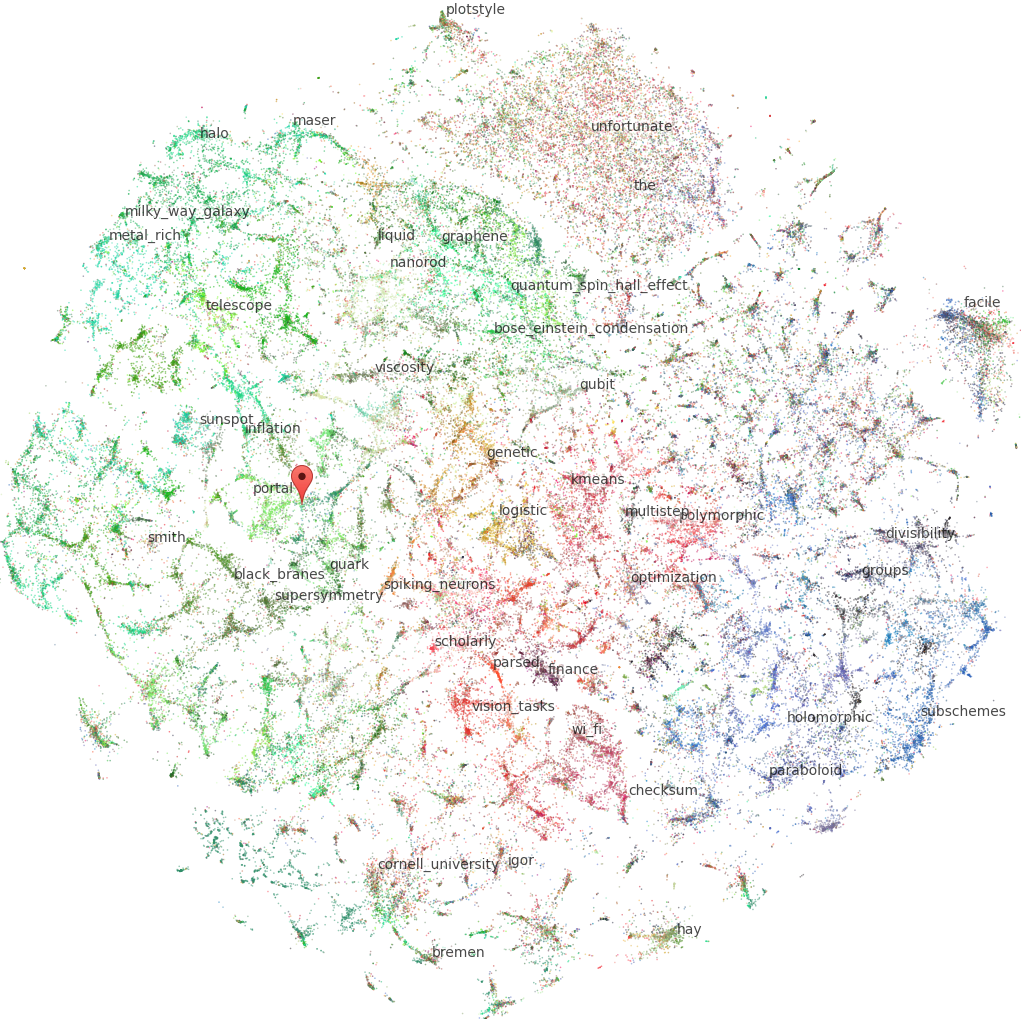
\includegraphics[width=.44\textwidth]{figs/ginsparg}
\caption{\small Embeddings of words appearing in scientific articles
posted on the arXiv, mapped from 200 to two dimensions using
t-SNE \citep{ginsparg}. Constructed using only three months of
arXiv articles, for a 130,000 word vocabulary---using more data
leads to better embeddings.
Interactive exploration of the embeddings
using a Google maps interface: \href{http://www.cs.cornell.edu/~ginsparg/arxiv/gmaps2.html}{cs.cornell.edu/~ginsparg/arxiv/gmaps2.html}.
}
    \label{fig:arxiv}
    \vskip2pt
\end{wrapfigure}

Fitting such models is difficult, and requires robust methods for
computation and evaluation.  Variational inference approximates the
posterior by fitting a family of distributions over the latent
variables to be close in Kullback-Leibler
divergence~\citep{Jordan:1999,Blei:2017}.  In the case of embeddings,
the variational distribution is $q(\alpha_{1:V}, \rho_{1:V} ; \nu)$
and we fit the variational parameters $\nu$ to be close in KL
divergence to $p(\alpha_{1:V}, \rho_{1:V} \g \mbx)$.  Recent
innovations in black box variational inference~\citep{Ranganath:2014},
probabilistic programming~\citep{Kucukelbir:2017,Tran:2017}, and
variational autoencoders
\citep{kingma} as implemented, for example, in Google TensorFlow, allow us to do this generically and
scalably, easily fitting many types of models to large
data sets.  This enables the exploration of many variants of the
models, e.g., different types of contexts, different values of $d$,
and different underlying conditional distributions. We will use
this framework to develop more advanced and useful embedding
algorithms, inspired by current knowledge of higher-level cognition.


\project{Representations beyond co-occurrence statistics}
Distributed embedding representations in machine learning are almost
exclusively based on co-occurrence statistics. For instance, when
constructing embeddings for words in text, names of colors (``red,''
``blue''...) will be embedded in nearby locations simply because they
tend to be used together. How can a richer knowledge of representation
in the brain be used to inspire algorithms for processing text,
images, and audio? As discussed above, the brain systems roughly
``embed'' as follows: visual cortex/appearance, frontotemporal
cortex/function, ventral striatum/reward, hippocampus/co-occurrence.
We will explore a wide variety of new machine learning models 
for representing data, using brain function as inspiration
for coding different aspects of data. For instance,
one embedding component learned in a reinforcement learning
setting might correspond to processing in the orbitofrontal cortext;
another embedding component based on semantic parsing of 
languages or scenes might correspond to processing in
the frontotemporal cortex. 
%Steps in such directions, have
%rguably made in recent work \citep{replearn}. 
The framework of exponential family embeddings and variational
inference provide powerful tools for this investigation.


\project{Embeddings for fMRI data}
In the other direction, from machine learning to cognitive
neuroscience, we believe that latent variable models and exponential family embeddings are
promising tools for advanced data analysis for fMRI.
[{\it Nick -- if you want to write a few sentences about the methodologies
that dominate fMRI analysis now, I can then try to comment on
how new machine learning methodologies might be applied.}]


\project{Time-dependent, multiscale representations}
As discussed above, known computational properties of the hippocampus
including pattern separation, different learning rates, and bridging
over time, have not yet entered the mainstream of machine learning.
We will study new learning architectures that attempt to mimic, even
if only as a computational metaphor, these capabilities in cognition.
To capture dependence on time, we will earlier work on dynamic topic
models~\citep{Blei:2006d}.  Dynamic topic models capture how the
latent themes in a collection can grow and shrink and change over
time.  By introducing multiple latent time series threads in such a
model, each having a different time scale, we can model different
learning rates in a dynamic model.  Dynamic topic models were
developed specifically for language.  We will generalize this idea to
capture the evolution over time of distributed representations.  In
the exponential family embedding framework, this amounts to placing a
linear dynamic prior on the embedding vectors or the context vectors,
or both.


\msection{Attentional Filtering (Objective 3) }
\label{sec:aim3}

More information is available to our senses than the brain can
handle. As a result, we process only a subset of this information and
this determines what enters conscious
awareness~\citep{Most:2005}, what we learn
~\citep{Turk-Browne:2005}, and what we store in
memory~\citep{Aly:2016}. The mechanisms governing the
selection of sensory information are referred to as the study of
\textit{attention}. An analogous problem, known as the curse of
dimensionality, arises in statistical machine learning for
high-dimensional problems. As with human attention, reducing the
dimensionality of data can make learning tractable. Here we will
explore whether our understanding of attention in cognitive
neuroscience can inform assumptions made in machine learning, and how
techniques for recovering lower-dimensional representations in machine
learning can be used to reconstruct fluctuations in human attention
from brain imaging data.

\biobackground{} Attention in the human brain can be controlled
reflexively by the salience of stimuli, including their 
contrast or motion~\citep{Itti:2000}. This
stimulus-driven, bottom-up form of attention explains how our focus
is automatically drawn to an approaching siren or to a screen
lighting up with a text message. It can be distinguished from
goal-directed, top-down attention, whereby we volitionally shift 
focus based on which stimuli are relevant for current behavioral
goals~\citep{Yantis:2000}. In both stimulus-driven and goal-directed
forms, attention is directed at external stimuli, enhancing evoked
activity in brain areas that code for their locations and
features~\citep{Kastner:2000} and increasing functional connectivity
between these areas~\citep{Turk-Browne:2013}. This modulation occurs
as a result of control structures in frontoparietal cortex that send
biasing signals to visual cortex~\citep{Noudoost:2010}. Attention can 
also be directed toward internal representations, such as
thoughts or memories, and this is mediated by similar
neural control mechanisms~\citep{Chun:2011}. This internal
attention, as well as goal-directed external attention, share the
fascinating property that are not determined by the appearance of the
world. Rather, they reflect computations in the mind and allow each
individual to process the same sensory input in different ways. The
challenge for understanding these forms of attentional filtering is
being able to characterize the inner mental life of a person, even in
cases where they do not (or cannot) disclose their focus.

Methods have been developed in recent years to infer
mental experience from brain data, including
colors~\citep{Brouwer:2009}, scenes~\citep{Naselaris:2009},
faces~\citep{Cowen:2014}, and locations~\citep{Sprague:2016}. These 
reconstruction or inverted encoding models
involve: (1) specifying a basis set of channels that tile the
dimension of interest; (2) for each stimulus, predicting the activation of each
channel given its v on
that dimension; (3) forva training set of fMRI data, modeling the
observed neural responses to these stimuli in each voxel as a weighted
sum of the predicted channel activations; (4) this results in an
estimated weight matrix of the extent to which each channel is encoded
in each voxel, from which a tuning curve for each voxel can be
computed as a weighted sum of the basis set; (5) by inverting this
estimated weight matrix, test fMRI data with the pattern of neural
responses across voxels for an unknown stimulus can be used to
estimate channel activation; (6) the weighted sum of these estimated
channel activations by the basis set provides a continuous readout of
the information present in the brain along the dimension of interest,
which can be used as is or for decoding by finding the stimulus whose
predicted channel activations (from step 2) are most correlated.

\setlength{\columnsep}{20pt}
\begin{wrapfigure}{R}{0.48\textwidth}
\centering
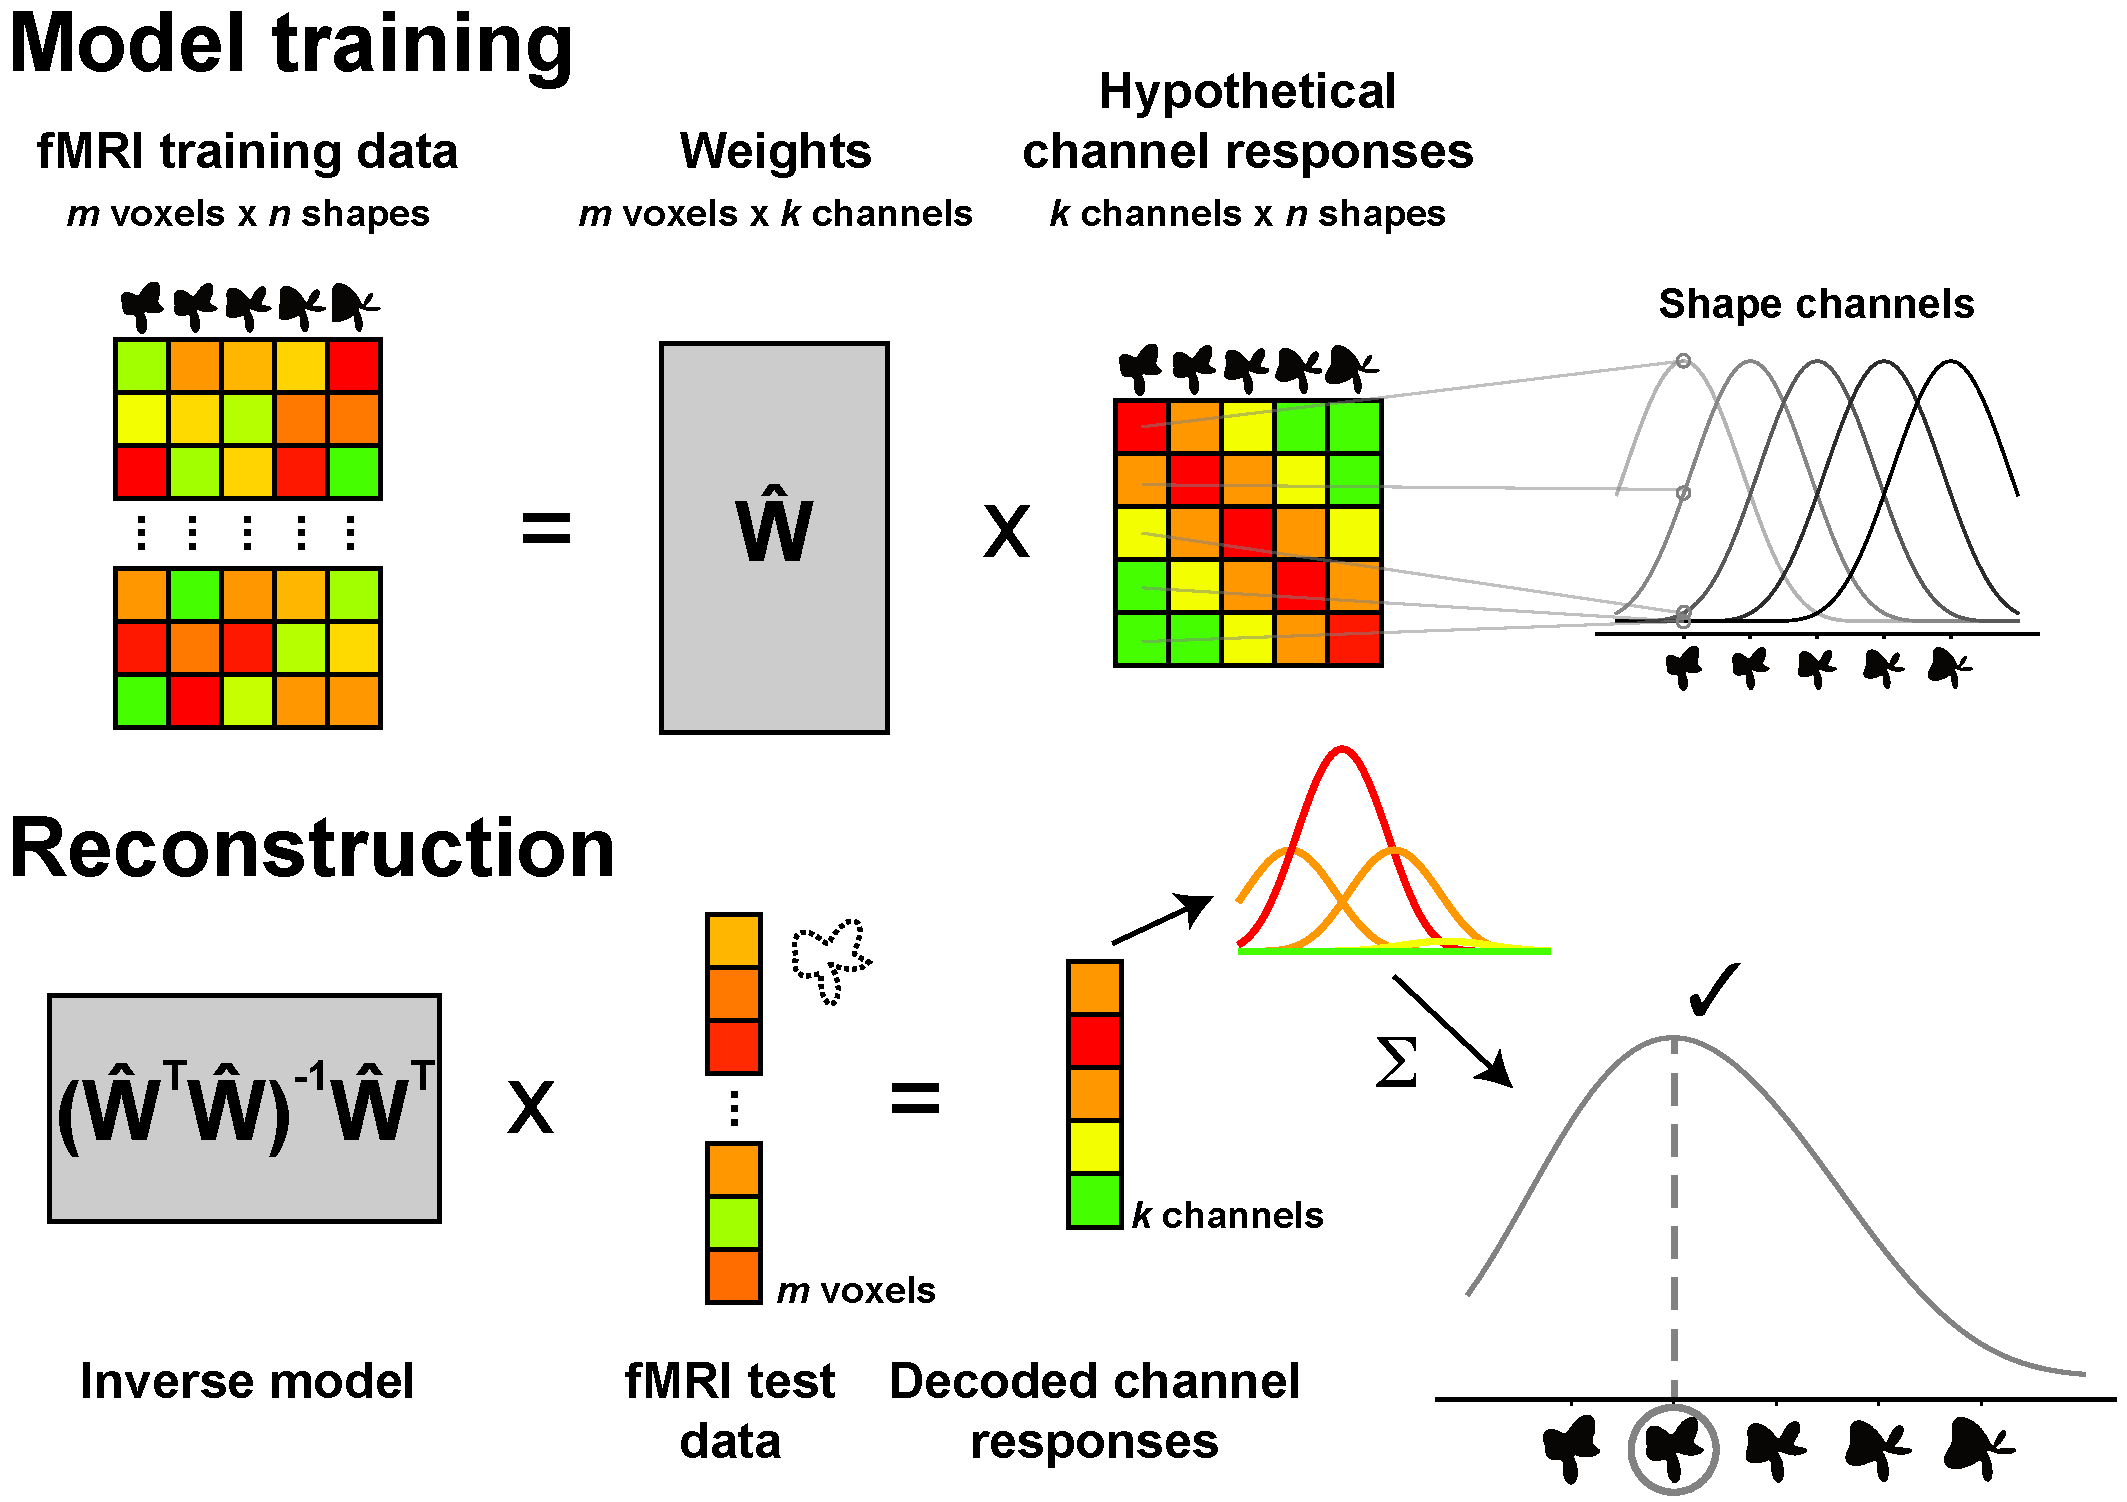
\includegraphics[width=.48\textwidth]{figs/inverse}
\caption{\small Example reconstruction analysis. Linear regression was
used to learn the tuning of voxels over a continuous space of novel
Fourier descriptor shapes. The inverse of the resulting weight matrix
was used to estimate the shape information present in a pattern of
activity over voxels in a brain region during a separate task in which
human subjects predicted which shape would appear on each trial.
In this study, shapes could be reconstructed from visual cortex and
hippocampus~\citep{Kok:2018}.}
    \label{fig:hippo}
    \vskip2pt
\end{wrapfigure}

Although these methods are cutting-edge and powerful in cognitive
neuroscience, and they come tantalizingly close to ''mind reading'',
they are currently limited in two ways. First, they require an
assumption (for training and decoding) that the brain veridically
represents the properties of the stimulus used as labels (e.g., known
visual or semantic features). To the extent that attention filters the
stimulus in some way, this changes the ground truth about which
features the brain should be representing, inherently limiting
reconstruction accuracy. Second, these methods are generally applied
to stimuli with one or a small number of potential dimensions that are
used for reconstruction. However, naturalistic stimuli are
high-dimensional and dynamic, increasing the likelihood that people
are shifting their attention between dimensions. We will thus extend
these approaches by attempting to reconstruct from brain activity not
only what stimulus information is present in each dimension but also
to which dimension(s) attention is directed. We will deploy methods
from machine learning that can uncover lower-dimensional traces
through high-dimensional data to infer how attention is filtering the
stimulus, even when the attentional focus during the training data is
unknown (i.e., it was not manipulated or measured). Our
overall goal is to improve decoding accuracy by reconstructing what is
represented in the mind rather than what is presented to the eyes.


\statbackground{} High-dimensional problems suffer from the curse of
dimensionality. This has a precise mathematical characterization in
standard models of statistical machine learning. The curse of
dimensionality has two components, one statistical, the other
computational. The statistical issue stems from the observation that
in high dimensions, any local ball will contain very few data
points. The computational curse is implied by the fact that searching
over a sufficiently large space of models is often
intractable. ``Beating'' the curse of dimensionality involves making
assumptions about the structure of the learning problem, and then
developing estimation and inference algorithms that provably 
recover that structure, with fast running times. The most prominent 
example in statistics in recent years is the assumption of sparsity, and the explosion of methods based on regularization that recover sparse signals \citep{Tibs:1996,lars,Wain:09a,wasserman:09,Zou:Hastie:Tibs:05,FHT:07}; methodology has also been developed for nonparametric problems \citep{LZ:Cosso,Ravikumar:08,lafferty2008rodeo,NPN:09,skeptic,NRRR:NIPS}

We will study mathematical formulations of attention as one approach
to making assumptions for which learning is tractable in principle.
In an attention-based model, the object of study is a
lower-dimensional trace or curve through the high-dimensional input
space. While the family of curves may be infinite dimensional, a
locally sparse or ``focused'' representation is intended to make
learning statistically and computationally tractable. Rudimentary
versions of this notion appear in the machine learning literature in
different forms.  For example, sparse coding representations have
been extended to be based on hierarchical and local coding schemes
\citep{WangYYLHG10,YuLL11}, and hierarchy and context have been 
incorporated into image models \citep{ChangJZBG11,JinG06}. In the
deep learning literature, attention-based models were first developed
in the setting of machine translation, using sequence-to-sequence
algorithms based on recurrent neural networks
(RNNs) \citep{bahdanau2014}. The attention mechanism is a type of
alignment model, which is a key component of statistical translation
methods \citep{Brown1993}. Attention has been applied to the problem of generating image
descriptions by \cite{showtell}.

\project{Attention-based latent embedding models}
We will investigate the introduction of the attention-based metaphor into
statistical learning using exponential family embedding models, latent
variables, and multiple embedding characteristics as described in
Objective 2 above. 
Recall from above that an exponential family embedding model uses a
latent representation of the input and output variables. Consider the
case of high dimensional density estimation, where the goal is to
estimate a density $p(x)$ for $x\in\reals^d$.  A latent variable
embedding model takes the form
$$ p(x) = \int p(z) \exp(\rho(x)^T \alpha(z) - \Psi_{\rho,\alpha}) \, dz$$
where $z\in \reals^m$ is a latent Gaussian vector,
$\rho:\reals^d \to \reals^K$ is an embedding of the input space,
and $\alpha: \reals^m \to\reals^K$ is an embedding of the latent
Gaussian, and $\Psi_{\rho,\alpha}$ is a normalizing constant.
In an attention-based model, we would consider a parameterized curve $t\mapsto (Z_t, S_t)$
where $Z_t$ is a Gaussian vector and $S_t \subset \{1,\ldots, d\}$
is a subset of the input variables. Define the inner product 
$\langle x, z\rangle_{\rho,\alpha}
= \int_{0}^1 \rho\left(x_{S(t)}\right)^T \alpha(Z_t) dt,$
and the corresponding embedding model
$ p(x) = \int \exp\left(\langle x, z\rangle_{\rho,\alpha} - \Psi_{\rho,\alpha}\right) d\mu(z)$ where $\mu(z)$ is a 
measure over ``attention paths,'' for example defined in terms of a Gaussian process.
In another version, consider a graph over $\{1,\ldots, d\}$ with edge
set $E$, and define the inner product
$\langle x, z\rangle_{\rho,\alpha}
= \sum_{(j,k)\in E} \rho(x_j, x_k)^T \alpha(Z_j, Z_k)$
where $Z$ is now a vector-valued Gaussian random field, 
and the model can be viewed as a nonparametric graphical model
\citep{hl18}. Returning to the discussion of data representation (Objective 2), 
if $Z(t)$ is an embedding having different components corresponding
to appearance, function, reward, and co-occurrence, then $S(t)$ might 
indicate attending to those different latent dimensions in turn.

These are thought of as attention-based models as the ``energy''
$\langle x, z\rangle_{\rho,\alpha}$ is localized to subsets of the
sample space or components of the latent variables. Discriminative or regression-based versions of these
models are defined similarly. The project will develop variational
inference algorithms for this family of models. When the mapping 
$\alpha(z)$ is defined in terms of, for instance, a feed-forward
neural network, this can be viewed in the framework of variational auto-encoders
\citep{kingma13}.


\project{Applications to fMRI movie data}
The public movie dataset mentioned earlier consists of 17 subjects
watching a 90-minute episode of BBC's Sherlock while being scanned with
fMRI~\citep{chen17,baldassano17}. We also have a frame-by-frame
annotation of several dimensions of the movie, including: scene
location, characters present, speaker, camera angle, music, arousal, and
valence (i.e., positive or negative mood). Consider the task of
reconstructing a person's subjective experience of the movie from their
brain data. As described above, existing inverse modeling methods
attempt to reproduce the visual or auditory stimulus presented to the
subject. However, for naturalistic stimuli like a movie with multiple
dimensions present, the limited capacity of human attention to a small
number of dimensions ensures that this reproduction will fail. We are
likely to only experience a subset of the input and which subset we
experience will change over time. There are currently no principled
techniques for characterizing this internal ''ground truth''. We will
exploit this annotated dataset to align the different dimensions of the
movie with the fMRI time series. Using an attention-based and dynamic
exponential family embedding model with multiple embeddings, we will
attempt to read out the attentional trace of the observer over time.


\project{Learning complexity under attention}
Classical statistical theory characterizes the complexity of
estimation and inference tasks in terms of minimax rates of
convergence. Parametric problems have risk (expected squared error)
that scales as $R_n \asymp p/n$ when there are $p$ parameters and $n$
samples. In the high dimensional sparse regime, research over the past
decade has shown that the risk scales as $R_n \asymp s \log p/n$ 
in a rich array of settings, where $s$ is the intrinsic dimension or
sparsity level. For nonparametric sparse additive
models \citep{Ravikumar:08}, it is known that the risk
scales (informally) as $\tilde O(s n^{-\alpha})$ where $n^{-\alpha}$ is 
the minimax rate for the underlying function space;
e.g., for an $m$-th order Sobolev space we have
$\alpha = 2m/(2m+1)$. These complexity results can be established using
the tools of empirical process theory, covering numbers, and metric
entropies. We will consider a series of mathematical formalizations
of attention, and investigate corresponding minimax rates of 
convergence, and bounds on approxmation errors in different settings.
As a concrete example, consider a regression model where the regression function 
has an attention component, expressed as 
$$ \E(Y\given x) = \int f(A_t^T x_{S_t}) \, dt.$$
This can be considered as a form of semiparametric single-index model
\citep{horowitz09,horowitz96,ichimura93,kakade11,negahban12} 
and we anticipate that we can characterize
the minimax complexity of estimating such models. We will also investigate
the theory of latent variable attention models.





 

\def\argmin{\mathop{arg\,min}}

\msection{Memory Capacity (Objective 4) }
\label{sec:aim4}

Given that the number of neurons and synapses in the brain is fixed,
to a first approximation, there must be a trade-off between the number of
memories that can be stored and the fidelity with which they are
stored. This is reflected in memory errors, interference, competition,
and decay. However, there is also evidence from human behavior that
people store a massive number of items in long-term memory with
incredible detail~\citep{Brady:2011}. How is this possible?
Computational architectures and insights could inform simple
experiments to better understand the nature of memory usage in living
systems. For example, recent work in deep learning has investigated
strategies for reducing memory usage. In the other direction, our
understanding of the way memories are stored in the brain can serve as
inspiration for computational and statistical models. In particular,
we will explore learning frameworks treating memory in terms of
inversion of generative processes.

\biobackground{}Human memory is a paradox, at once exquisite, as when
a photograph transports us back through time to relive a past event,
and at other times elusive and unreliable, as when trying to recall a
colleague's name. Indeed, most cognitive neuroscience research on
human memory views it as adaptively fallible and
distorted~\citep{Schacter:2011}. Unlike a hard drive, related
memories overlap and interact with each other in the brain even when
supposedly dormant, leading to the creation of false memories and forgetting of competing memories~\citep{Kim:2014,Wimber:2015}. In
this context, it is surprising that
humans~\citep{Standing:1973,Brady:2008} and non-human
primates~\citep{Woloszyn:2012,Meyer:2018} can remember
hundreds or thousands of visual images with remarkable detail. For
example, ~\citet{Brady:2008} presented human subjects with 2,500
objects for 3 s each. Memory was tested afterward by having them
choose which of two objects presented on each trial had been studied
before. Critically, one of the objects was an exact match to earlier
(i.e., familiar target) and the other object (i.e., novel foil) varied
in similarity to the target. If the studied objects remained in
memory despite long delays and many intervening items, subjects
should reliably choose the target. Insofar as these memories
are detailed and precise, accuracy should be high even when the novel
foil was highly similar to the target (e.g., if the target
was a breadbox with a loaf of bread inside, a highly similar ''state
change'' foil would be the same breadbox and loaf, but with the loaf
sitting in front). Indeed, accuracy on such trials was 87\% on average
relative to 50\% chance, for thousands of objects seen once, which was
only a little worse than if the foil (93\%) was completely unrelated
and coarser memory would suffice (e.g., breadbox vs. remote control).

These kinds of detailed, one-shot (or \textit{episodic}) memories,
formed within minutes or hours, are thought to be initially dependent
on the hippocampus (see Objective 2). This raises the question of how
such a small mass of tissue is able to store thousands of images in a
short time without much loss in precision. Indeed, the problem of the
storage capacity of the hippocampus has been studied for a long time.
For example, ~\citet{Marr:1971} argued that 100,000 memories could be
stored there, corresponding roughly to the number of seconds in a day,
and that these memories would be offloaded to higher-capacity
neocortex during sleep each night, resetting the counter. There are
several possible solutions to this problem, including reducing the
number of units used for each memory (i.e., sparse coding), increasing
the number of units available for representation, or accelerating
forgetting and decay~\citep{McNaughton:1987}, as well as by expanding
the building blocks and sites of memory beyond synapses to include
biochemical cascades~\citep{Fusi:2005}. More generally, theoretical
estimates of the storage capacity of neural networks with distributed
memories suggest that it is a fraction of the number of units
and also depends on connectivity~\citep{Hopfield:1982,Brunel:2016}.

\statbackground{} Memory is a foundational theme throughout the broad
landscape computation. In information theory, the notion of memory was
probed in Shannon's landmark paper, which presaged hidden Markov
models in the discussion of finite state models of language, with a
state representing the ``residue of influence'' of the previous
letters \citep{Shannon:48}. A rich mathematical literature exists that
explores the mathematical properties of finite and infinite stochastic
processes with respect to notions of memory, including mixing
properties of chains \citep{pollard84}. Popular neural network models
for more flexibly handling long-range dependence include LSTMs and
their variants \citep{sepp97,gers00}. This latter work serves to
remind us that even simple metaphors for learning in humans, when
implemented in scalable and easily available code, can lead to methods
having great impact in contemporary applications.

Recent work in deep learning has investigated
strategies for reducing memory usage \citep{ChenXZG16}. During a
forward pass, only a subset of the nodes' activations are kept in
memory, and the others are discarded. In back-propagation, the
computation is redone at the forgotten nodes. This induces a trade-off
between time complexity and memory. The practical problem is to
determine the subset of nodes to checkpoint, given the network and a
memory budget. The tradeoff can be thought of in terms a simple pebble
game.  Other work on tradeoffs in statistical learning includes
\citep{lucic15tradeoffs}. Insights from neuroscience could inform novel algorithms for reducing
memory in artificial learning algorithms.

Work over the past 3-5 years has analyzed a range nonconvex
optimization problems, including phase retrieval, compressed
sensing under sparsity constraints, low-rank matrix
completion, and randomized sensing of low rank matrices
\cite{phaselift_1,phaselift_2,phaselift_3,ZhaWanLiu15,WeiCaiCha16,ZheLaf15,phaselift_1,phaselift_2,phaselift_3,ZhaWanLiu15,WeiCaiCha16}.
Some of this work demonstrates that the local optima are either
non-existent, or can be avoided by simple initialization schemes. Many
of the results make assumptions of random problem instances.  Very
recent work has established technical results toward showing it is
possible to invert randomly constructed deep networks. For example,
\cite{HandV17} consider networks that compose multiple ReLU-transformed affine
maps, which is a simple but often practically effective deep learning
architecture.  
\cite{HandV17} show that the inversion objective function for such networks, based
on empirical risk minimization, does not have spurious stationary
points, so that at any point away from an optimal solution has a
descent direction. The related results of \cite{Mixon18} make use of
the machinery of spherical harmonics and Gegengauer polynomials for
establishing inversion algorithms for certain two-layer
networks. Together with more recent results of \cite{HandV18}, this
line of work begins to establish compressed sensing theory for a rich
family of generative models.

% generative models as memory
% hand, voroninski
% optimization with backtracking memories
% risk bounds as a function of memory in density estimation

\project{Nonparametric estimation with memory constraints}
As discussed in Section~2, recent work has established 
sharp constrained minimax analysis of nonparametric
regression under quantization and communication
constraints \citep{Zhu:18,Zhu:18b}; related results are shown
for wavelets and Besov spaces \citep{szabo18}.
It is of interest to understand how memory restrictions might affect
statistical rates of convergence. While this earlier work focuses on
normal means formulations, a more practical framework for
nonparametric estimation is local averaging using kernels. In
classical theory, the actual form of the kernel does not affect the
rate of convergence, as it enters as a constant in the bias and
variance calculations. However, the kernel can be viewed as a
simple formalization of memory---a kernel evaluation $K(x,x')$ asks
``how similar is the current stimulus $x$ to a previous stimulus $x'$
observed in my past experience?'' We will consider mathematical models for
how the kernel $K$ degrades under memory constraints that
are motivated by empirical findings in cognitive neuroscience,
and derive minimax results under such memory constraints. The
Tsybakov low-noise condition will be used to allow for
high-dimensional learning \citep{mammen1999,tsybakov2004,audibert2007}.



\project{Inversion of nonconvex generative models using memory landmarks}
Many practical systems are constructed with deep convolutional
networks using ReLUs; these represent hierarchical compression
schemes. Their corresponding generative counterparts are ``decoder
networks'' which take a dense Gaussian input and expand it to, for
example, a synthetic image.  We will study models of memory in
cognition that are based on inverting generative/decoder networks. The
recent of work of \cite{HandV17} (see also \cite{HandV18}) shows that
if $G(z)$ is such a network with random weights, and $A$ is a random
matrix, then the empirical risk function $ f_x(z) = \|AG(z) -
Ax\|_2^2$ is remarkably well-behaved. Specifically, under natural
conditions on the scaling of the network size, the function $f_x(z)$
has no local optima or critical points (outside of two neighborhoods
around the optima). We will investigate computational questions in
this setting motivated by simplified notions of memory, plasticity and
learning in the brain. In particular, suppose that the weight matrices
of such a network are initialized randomly; thus every point has a
descent direction. As the network is fed data, the weight matrices are
optimized to learn to code for those data.  During this learning
phase, where the network weights are reconfigured (plasticity), they
become nonrandom, and the function $f_x(z)$ becomes highly
nonconvex. We will study algorithmic techniques where the descent
directions at intermediate points are remembered (or ``memoized'')
during this learning phase. As the landscape becomes highly nonconvex,
these previous descent directions are landmarks used for searching and
decoding the nonconvex objective by gradient descent. The learned
decoder is used to assess future data against past experience.


\msection{Relation to TRIPODS Project}

Brown's TRIPODS award, \emph{Foundations of Model Driven Discovery from Massive Data}, focuses on the interplay between the analysis of data arising from a coherent data generating model or mechanism and the refini of such models from tools in data analysis. The focus areas of Brown's TRIPODS activities include, causal inference, graphs and networks, and geometry and topology of data. Each of these areas fits thematically with the proposed project and its objectives.

The activities supported by the TRIPODS award include intensive visits, Seminars, and Summer or Winter Schools, each of which will naturally support the theme of the proposed project, as a ``research domain'' to which methods in each TRIPODS focus area can fruitfully be applied. The proposed activities involve visits between teams of researchers and their students at Yale and at Brown, naturally dovetailing with proposed activities in the TRIPODS project. 
\msection{Broader Impact}

This proposal reflects the first, to our knowledge, structured
partnership between neuroscience and data science at Yale, and likewise the first between Brown's Data Science Initiative and its neuroscience community as such. The partnership
presents many new opportunities for promoting teaching, training, and
learning: First, the project will support two graduate students, one in
Psychology and the other in Statistics \& Data Science (S\&DS). They will
work in close coordination with senior personnel from both neuroscience
and data science, to gain mastery of both fields and to serve as a vital intellectual bridge. Second, several other
graduate students at Yale and Brown will participate in research
projects, workshops, and annual exchanges between institutions to learn
from other researchers and the communities. Third, neuroscience and data
science are the two newest undergraduate majors in Yale College, and the
assembled team is deeply invested in these programs (e.g., Turk-Browne
and Clark serve as co-directors of the neuroscience major). This project
will facilitate interaction between the majors, including a data science
course with neuroscience lab (Lafferty) and a neuroscience course
teaching data science approaches (Turk-Browne). These courses will be
cross-listed and coordinated so interested students can take both.
Fourth, seniors in our departments complete a year of independent
research. The project objectives provide opportunities for at least four
undergraduates per year to gain cutting-edge research experience. Joint
training in our fields is invaluable preparation for the STEM workforce,
where computational and mathematical skills paired with domain knowledge
in behavior, neuroscience, and artificial intelligence are highly sought
after. Fifth, the two workshops we organize, at Yale in year 1 on
neuroscience challenges and at Brown in year 2 on data science methods, will be geared at an accessible level and open to students and faculty on campus, to build
a broader community.

This collaboration involves an unusually broad constellation of people,
expertise, methods, and resources. Thus, the project activities will
enhance infrastructure for research and education in several ways:
First, the project will bring together four departments at Yale that
have not traditionally had substantive interactions: Psychology
(Turk-Browne), Molecular, Cellular, \& Developmental Biology (Clark),
Statistics and Data Science (Lafferty), Computer Science (Lafferty), and Mathematics (Brock). 
Second, it will establish a
new bridge between Yale and Brown, institutions that are relatively
nearby (short train ride away) and that have made significant
investments in neuroscience and data science. Combining forces, in terms
of faculty interaction and student exchanges, will multiply the impact
of these initiatives, and we hope lead to a new regional network focused on
\emph{data neuroscience}. Third, there are many relevant efforts underway on
each campus with which we can partner to further realize value from this
project. At Yale, these include: the Yale Center for Research Computing,
which manages centralized clusters and offers boot camps in scientific
programming, parallel computing, and software development; the human
brain imaging center in the Faculty of Arts and Science (overseen by
Turk-Browne) that will open this fall next to Psychology and S\&DS,
providing training for FAS students and faculty on how to conduct fMRI
studies and generous funding to enable studies without external grant
support; and the Quantitative Biology Institute (Q-Bio), an hub of
computational scientists (including Clark) that will provide additional
research opportunities. At Brown, relevant initiatives include: the NSF
EPSCoR Attention Consortium (Sheinberg is Co-PI), a multi-institution
effort to develop a unified model of attention, relevant to some of the
proposed research; the NSF-funded Institute for Computational and
Experimental Research in Mathematics (ICERM), which bridged mathematics
and computation (with founding co-PI's Brock and Sandstede serving as inaugural Deputy and Associate Director respectively);
and the Data Science Initiative (DSI) in which TRIPODS sits (Brock is
Director, followed by Sandstede this summer) to be co-located in new space with Brown's Carney Institute for Brain Science in January 2019. Fourth, the activities supported by
this project have relevance to the technology industry, creating
opportunities for new partnerships and dissemination. As an example,
Turk-Browne has been a core member of a partnership with Intel Labs
started in 2015 that funds academic research and researchers in advanced
fMRI analysis, but also led to the creation of an internal group at
Intel Labs devoted to brain-inspired computing and intelligence.



\msection{Results from Prior NSF Support}

\textbf{Nick Turk-Browne} was previously supported as co-PI under NSF
grant BCS-1229597, ``MRI: Acquisition of High Performance Compute Cluster for Multivariate Real-time and Whole-brain Correlation Analysis of fMRI Data'' from August 15, 2012 to July 31, 2015. The PI of the grant was Jonathan Cohen and the co-PIs were Ray Lee, Kai Li, Kenneth Norman, and Turk-Browne (all Princeton University at the time). The total award amount was \$527,978.

{\bf Intellectual Merit.} This project resulted in the acquisition of a high-performance compute cluster for the analysis of human brain imaging data, installed in the Princeton Neuroscience Institute (PNI). The cluster consisted of 50 nodes, each with dual E5-2670 Xeon chips (16 CPU cores) as host CPUs and 2 Xeon Phi 5110P boards (120 CPU cores) as primary compute nodes, with 256GB DRAM, 1.6TB Flash memory, 30TB of local storage and 10GbE network interface (6,800 cores total). The Xeon and Phi processors were donated by Intel Corporation as in-kind cost sharing, valued as a similar amount to the award from NSF. This system was integrated with state-of-the-art functional magnetic resonance imaging (fMRI) equipment at PNI, enabling two exciting long-term projects that required rapid-throughput analysis of high-dimensionality data: closed-loop real-time neurofeedback and whole-brain functional connectivity analysis. It resulted in several publications, including ~\citep{Cohen:2017,deBettencourt:2015,Turk-Browne:2013,Wang:2015}.

{\bf Broader Impact.} This work brought together a diverse team of neuroscientists, psychologists, physicists, and computer scientists, enhancing not only the computing and imaging infrastructure at Princeton, but also its intellectual and educational environment. Many graduate students, postdoctoral fellows, and faculty have used this cluster for neuroscience research. This includes the neuroscience and computer science graduate students deBettencourt and Wang, who led each of the projects mentioned above, respectively, resulting in first-authored publications. These projects also resulted in the development of BrainIAK, a high-performance open-source software package for advanced fMRI analysis, as part of an industry partnership with Intel Labs (brainiak.org).

\vskip10pt \noindent Turk-Browne was previously Co-PI of NSF grant
ACI-1440750, ``CC*IIE Engineer: A Software-Defined Campus Network for Big-Data Sciences'' from September 1, 2014 to Auguest 31, 2016. The PI of the grant was Jennifer Rexford and the co-PIs were Curt Hillegas, Christopher Tully, and Turk-Browne (all Princeton University at the time). The total award amount was \$399,776.

{\bf Intellectual Merit.} This project resulted in the hiring of a full-time cyber infrastructure engineer (CIE), who has been leading a major campus initiative to deploy software-defined networking (SDN) for the next generation of data-driven scientific research, including in neuroscience, physics, geosciences, and genomics. This initiative led to cost-effective scaling of the campus IPS, innovative solutions to server load balancing, better monitoring of network performance with perSONAR, and testing of OpenFlow switches.

{\bf Broader Impact.} One of the first tasks of the CIE was to create a survey that interviewed faculty about their networking needs. This survey and subsequent activities under this project led to a unique collaboration between researchers in Computer Science and the administrative Office of Information Technology, helping ensure that academic research needs across campus were central to IT infrastructure decisions.

\vskip10pt \textbf{John Lafferty} was previously supported as co-PI under NSF
grant IIS-1116730, ``III: Small: Nonparametric Structure Learning for
Complex Scientific Datasets,'' from August 1, 2011 to July 31, 2014.
The PI of the grant was Han Liu (Princeton University) and the co-PIs
were Lafferty and Larry Wasserman (Carnegie Mellon University).  The
total award amount was \$499,344; the amount awarded to the University
of Chicago was \$118,750.

{\bf Intellectual Merit.} %The research supported under this grant
%contributed to the subfield of statistics called nonparametric
%sparsity, which exploits novel sparsity-inducing regularizations to
%fit nonparametric models. The project focused on developing scalable
methods for finding structure in complex scientific datasets, without
making strong distributional assumptions. The project explored several
aspects of nonparametric structure learning, including methods,
theory, large-scale computing, and applications, with five concrete
aims: (1) nonparametric structure learning in high dimensions, (2)
nonparametric conditional structure learning, (3) regularization
parameter selection, (4) parallel and online nonparametric learning,
and (5) minimax theory for nonparametric structure learning problems. 
The outcomes included practical models and algorithms; application
areas included genomics, cognitive neuroscience, climate science,
astrophysics, and language processing.  Publications resulting from
this grant include
\citep{fcca,mehddtgm,chen:13,challenges,quadro,bigp,admm,NRRR:NIPS,gu:
12,ospif,hdssipca,tpca,pcangd,rspcr,tmehdv,scale,pca,bernoulli,direct,
coda,spcahdmts,peace,cna,biglasso,fshdc,kolarhan,gemad,gemd,
lafferty2012,flare,hdtgm,liu2012,skeptic,expoconc,insensitive,mrc,
eigens,calibrate,blossom,Mishra:2015,patterns,mngm,fclime,joint,retm,
tests,shender:13,soft,latenttree,tar,sconvex,xu:14,csc,sicec,
calibratedp,huge,hdngevspnp,semirank,amrbcdm,qnegsm,Zhu:18}.

{\bf Broader Impact.} The broader impact of the project included
interdisciplinary training for graduate students from biostatistics,
computer science, statistics, and medical schools, strengthening the
collaboration and interdisciplinary infrastructure between Carnegie
Mellon, Johns Hopkins, the University of Chicago and Princeton, and
broadly disseminating the results from this research in journals from
all relevant fields. The research had impact outside of machine
learning and statistics. In a genomic study, PI Liu applied structured
nonparametric methods to analyze high dimensional genomic data,
identifying several gene mutations associated with autism.  These
results were published in Nature \citep{patterns}, and reported in the
New York Times. In another neuroscience study, the PI developed an
effective algorithm for predicting Attention Deficit Hyperactive
Disorder (ADHD) disease.  The research led to several statistical
software packages in R, including \citep{huge,fclime,flare}, all of
which are freely available on CRAN.

\vskip10pt \noindent Lafferty is currently supported as PI under NSF
grant DMS-1513594, ``Constrained Statistical Estimation and Inference:
Theory, Algorithms and Applications,'' from June 29, 2015 to July 1,
2018. The total award amount was \$320,000. After two years of the
project, the remainder of the funds were transferred from the
University of Chicago to Yale University, where the PI moved in July
2017.

{\bf Intellectual Merit.}  The project is studying constraints that
are present in complex scientific data analysis problems, but that
have not been thoroughly studied in traditional approaches. Different
aspects of theory, algorithms, and applications of statistical
procedures, with constraints imposed on the storage, runtime, shape,
energy or physics of the estimators and applications. The overall goal
of the research is to develop theory and tools that can help
scientists to conduct more effective data analysis. Publications under
this grant have included \citep{ChatterjeeL18,MishraILH18,
abs-1803-01302,MishraLH17,YangB0L16,ChatterjeeDLZ16,ZhengL16,
MishraZLH15,ZhengL15,ZhuL14,Bonak18}


{\bf Broader Impact.} The broader impact of the project is aimed in
three directions. First is the development of flexible and principled
large scale data analysis tools that can benefit many scientific
domains.  Second, is the development of software that is widely
distributed, allowing others to build on the work. The third is to
education, to allow the research to impact the training of students at
both the graduate and undergraduate levels.


\vskip10pt \noindent Lafferty was previously PI of NSF grant
DMS-1547396, ``RTG: Computational and Applied Mathematics in
Statistical Science'' from July 1, 2016 to July 1, 2017. This grant
did not transfer to Yale University; the current PI is Jonathan Weare
at the University of Chicago. The total award amount is \$1,697,320.

{\bf Intellectual Merit.}  This Research Training Group (RTG) project
supports creation of a dynamic, interactive, and vertically integrated
community of students and researchers working together in
computational and applied mathematics and statistics. The work is
motivated by the growing need to train the next generation of
statisticians and computational and applied mathematicians in new
ways, to confront data-centric problems in the natural and social
sciences.

{\bf Broader Impact.} The broader impact includes vertical integration
of education and training from undergraduate to postdoctoral
researchers, including activities at Toyota Technological Institute at
Chicago and Argonne National Laboratory. Participants in the RTG will
receive an educational experience that provides them with strong
preparation for positions in industry, government, and academics, with
an ability to adopt approaches to problem solving that are drawn from
across the computational, mathematical, and statistical sciences.

\vskip10pt \textbf{Damon Clark} is currently supported as PI under NSF
grant IOS-1558103, ''Understanding how Neural Nonlinearities Tune
Motion Detection in the Fly Eye,'' from July 1, 2016 to June 30, 2019.
The total award amount is \$461,262.

{\bf Intellectual Merit.} This project focuses on the nonlinearity
associated with visual motion detection circuits in fruit flies. Our
aims are to characterize that nonlinearity with behavioral and neural
measurements, dissect how individual neurons in the circuit contribute
to it, and investigate how that nonlinearity relates to the
performance of the circuit with naturalistic inputs. We have so far
published a review~\citep{clark:16} and a methods
paper~\citep{mano:17}, and currently have three more manuscripts
submitted or under review.

{\bf Broader Impact.} We have had 3 high school students work in lab
over the summers (2016-2018), and completed lessons in Yale's
\textit{Pathways to Science} program that focused on what visual
illusions teach us about how the brain works.

\msection{Results from TRIPODS Project}

\textbf{Jeff Brock} is currently supported as PI under NSF TRIPODS grant CCF-1740741, ''Foundations of Model Driven Discovery from Massive Data,'' from September 1, 2017 to August 31, 2020. The co-PIs of the grant are Stuart Geman, Eli Upfal, Bjorn Sandstede, and Joseph Hogan (Brown University). The total award amount was \$1,482,177.

The TRIPODS grant, in its first year, sought to bring researchers from diverse communities together for workshop activities, and likewise engaged remote researchers to come to campus for seminar talks and research engagement with affiliated faculty and students. We have recently hired 3 postdoctoral fellows to start on July 1, who will assist with achieving the goals of the project.

A fall 2017 workshop entitled Geometry and Topology of Data took place at ICERM in December 2017. This workshop was intended to bridge communities working in Topological Data Analysis, and methods of Diffusion Geometry to study high dimensional data sets. Impacts from workshop were extensive, leading to future collaborations that are the topic of three of our TRIPODS + X proposals, in neuroscience, in data science education, and in gene regulatory networks. We are tracking collaborations going forward, but list one paper of Oudot and Solomon, on which Oudot spoke at the conference (arXiv:1712.03630).

Brown's TRIPODS Institute has been focused on developing models for center related activities that build on intensive visits from outside scientists working in the focus areas of the Institute. In particular, the TRIPODS Institute sponsored short visits from researchers in the theme of topological data analysis to the TRIPODS sponsored Applied Topology Seminar. Highlights include visits from, Justin Curry, Attila Gyulassy, Lori Ziegelmeier, Carina Curto, Steve Oudot, Anthea Monod and Andrew Blumberg.

{\bf Training Activities.}
The visit from Oudot, of INRIA, served further the collaboration with Brock's graduate student Isaac Solomon. Oudot spoke on their work at the workshop, and Solomon is speaking at the Ohio State TRIPODS workshop on their joint work in late May 2018. According to Solomon, ''The general goal of our project is to use techniques from applied topology to analyze intrinsic metric structures, in particular metric graphs... Steve presented our ongoing work at the workshop, and I have presented on it at various conferences, including the upcoming TRIPODS workshop at Ohio next week.''

Sandstede's student Melissa McGuirl met with many of the TRIPODS visitors, who provided valuable research insights as well as career mentorship. In particular, she met with her co-Advisor, Blumberg, from U. Texas to discuss her thesis work. McGuirl also had substantial interactions with many of the speakers including Gyulassy of whom she says, ''We met to discuss ways to extract features from images. In particular we talked about Morse theory applications. We also discussed the current software tools available for this method.''

The PI has engaged in planning a week long summer bootcamp with Solomon, McGuirl, and Henry Adams of Colorado State, who will spend a week in early August presenting the framework of topological data analysis in the context of machine learning. This weeklong workshop (to run at ICERM) will focus on bringing graduate students up to speed with the tools and techniques of TDA, and bring in outside speakers to present their applications in to machine learning.

Finally, the TRIPODS Institute will sponsor a two day workshop in mid-August on building community in theoretical foundations of data science, focused on regional collaboration and interaction between researchers in the theoretical aspects of data science.


%-----------------------------------------------------
\clearpage
\setcounter{page}{1}

\renewcommand{\refname}{References Cited}
\bibliography{3podx,3podx-clark,3podx-representation,jdl-previous,vision,hippocampus,prior-ntb,attention,memory}

%-----------------------------------------------------
\clearpage
\setcounter{page}{1}
\def\person#1{\vskip4pt\noindent{\it\bfseries #1}}
\let\blurb\person

\section*{Project Coordination Plan}

\person{Roles and responsibilities}: This proposal includes eight key
personnel, evenly divided between data science and neuroscience, and
between Yale and Brown, the latter being the home of a TRIPODS
institute. The TRIPODS+X solicitation initiated conversations that led
to this proposal. In preparing it, we discovered previously unrealized
connections and shared interests within Yale and between Yale and
Brown. As such, funding this proposal will provide resources needed to
launch a new interdisciplinary collaboration at the intersection of
data science and neuroscience that would otherwise not be possible.

\person{Nick Turk-Browne} is a cognitive neuroscientist at Yale and will serve
as the lead PI. He will be responsible for administrative oversight of
the project, including being the contact for NSF, reviewing the budget
and expenditures quarterly, and preparing reports. His technical
responsibilities will be to procure existing fMRI datasets, format and
preprocess these data, and develop software packages that implement
current and new fMRI analysis tools (e.g., \href{http://www.brainiak.org}{brainiak.org}). His
scientific responsibilities will include mentoring a graduate student
in neuroscience and generating hypotheses and models of
representation, attention, and memory (objectives 2-4, respectively)
and interpreting findings based on theories of human brain function.


\person{John Lafferty} is a data scientist at Yale and will serve as Co-PI. He
will be responsible for leading the data science aspects of the
project (in all objectives). This includes lending his expertise in
machine learning, identifying and creating relevant algorithms,
developing precise mathematical formulations, and considering how
principles of the brain could be imported to enhance approaches in
data science. He will mentor a graduate student in data science and
teach a neuroscience lab as part of a new data science course.

\person{Damon Clark} is a cellular and computational neuroscientist at Yale and
will serve as Co-PI. He will be responsible for providing and
analyzing neuronal recordings from {\it Drosophila} and for developing
computational models of circuit function (objective 1). He will
co-supervise the graduate student in neuroscience so that s/he can
learn how computational principles apply across different species'
brains.

\person{Jeffrey Brock} is a mathematician and currently PI for the
TRIPODS grant at Brown. He will join Yale's faculty with an appointment as Professor of Mathematics on July 1 and as Dean
of Science on January 1, 2019. His role will transition to Co-PI for the TRIPODS
grant at Brown. He will serve as Co-PI on this project, responsible for
close coordination with the aims of TRIPODS, focusing in particular on geometric and topological methods in analysis of neural data and identifying mathematical
concepts relevant to the objectives of this project. He will also serve as the key liaison to the Brown
TRIPODS PI team. He will co-supervise the graduate student in data
science to ensure that s/he learns about other application domains.

\person{Marvin Chun} is a cognitive neuroscientist at Yale and will serve as
Faculty Associate. He will be responsible for lending expertise in
human attention and memory (objectives 3-4, respectively) and
particularly the use of reconstruction models in fMRI analysis.

\person{Bjorn Sandstede} is an applied mathematician at Brown and will serve as
Faculty Associate. He will become PI of the TRIPODS grant at Brown. He will
be the primary contact at Brown, responsible for coordinating that
team of faculty and students. He has also worked on fMRI connectivity
and causal inference from networks and so will play an active
scientific role in the work on attentional filtering (objective 3).

\person{Stu Geman} is an applied mathematician at Brown and will serve as
Faculty Associate. He is a world expert in shape recognition and will be responsible for lending expertise in neural coding (central to objectives 2 and 4).

\person{David Sheinberg} is a systems neuroscientist at Brown and will serve as
Faculty Associate. As an expert in non-human primates, who exhibit
similar behaviors to humans but allow for invasive recordings as in
{\it Drosophila}, he will serve to bridge across objectives and
techniques. His scientific focus on perception, attention, and memory
will benefit many of the proposed research activities.

\person{Expertise in neuroscience}: The ``X'' application in this application is
represented extremely well by the team of four neuroscientists above
(Turk-Browne, Clark, Chun, Sheinberg). We cover the spectrum of model
systems (humans, monkeys, flies). We employ most modern
neuroscientific techniques (neuronal recordings, optogenetics and
stimulation, cellular and whole-brain imaging, brain-damaged patients,
neural network modeling). We have continuous funding for neuroscience
research from NIH and/or NSF. We serve on editorial boards, advisory
boards, and grant panels for neuroscience research. Our labs give
multiple conference presentations every year at neuroscience
conferences like SfN. We have appointments, teach, and mentor students
in neuroscience graduate programs. Two of us (Turk-Browne and Clark)
are the co-directors of the neuroscience major at Yale. To go into
more detail about the PI (Turk-Browne), he has published 35
peer-reviewed articles containing one or more fMRI studies. He has
received major funding from NIH (2 R01s), NSF, Templeton Foundation,
and Intel Labs in support of his fMRI research. He has received 6
early career contribution awards, including from the Cognitive
Neuroscience Society. He has pioneered new fMRI approaches, including
background connectivity, closed-loop neurofeedback, full correlation
matrix analysis, hippocampal segmentation, and imaging of awake and
behaving infants. He has trained 7 PhD students and 6 postdocs in
cognitive neuroscience (10 of whom hold faculty positions, including
at: UBC, UPenn, UCSD, Oregon, Columbia, UCL). He has a track record of
interdisciplinary collaboration, including with computational
researchers in systems, networking, and machine learning. 

\blurb{Managing the collaboration}: The PI, Co-PIs, and Sandstede will
comprise an executive committee that will meet monthly. Turk-Browne
will be responsible for managing cognitive neuroscience activities,
Lafferty for data science activities, Clark for cellular neuroscience
activities, Brock for coordinating with TRIPODS, and Sandstede for
leading the Brown team. This committee will review project progress,
identify areas for improvement, make strategic personnel and research
decisions, resolve conflicts, and work toward long-term funding. The
regular interaction and proximity of Yale researchers (all within 2
blocks) and the close ties between Brock at Yale and Brown personnel
will ensure responsible execution of this project.

\blurb{Coordination mechanisms}: We envision four mechanisms to learn from
each other and to make progress on project objectives: (1) a weekly
Zoom videoconference with faculty and students, involving a business
meeting followed by a scientific presentation; (2) annual exchanges
for a few days of 4 Brown students to Yale and 4 Yale students to
Brown; (3) a workshop at Yale in year 1 focused on neuroscience; (4) a
workshop at Brown in year 2 focused on data science. Each workshop
will begin with activities that introduce the kinds of data and
methods unique to the project and discipline, at a level suitable for
graduate students. This will be followed by a series of lectures by
more senior personnel explaining the active work and progress along
the various objectives. The workshops will be designed to invite
others on campus to build community. Funding for the exchanges and
workshops is included in the proposed budget.


\def\graycell{\cellcolor[RGB]{200,200,200}}
\def\acell{\cellcolor[rgb]{.98,.81,.69}}
\def\bcell{\cellcolor[rgb]{0.54, 0.81, 0.94}}
\def\ccell{\cellcolor[rgb]{0.98, 0.91, 0.71}}
\def\dcell{\cellcolor[rgb]{0.64, 0.76, 0.68}}
\def\ecell{\cellcolor[rgb]{0.96, 0.76, 0.76}}
\def\g{}
\def\g{\graycell}
\def\a{\acell}
\def\b{\bcell}
\def\c{\ccell}
\def\d{\dcell}
\def\e{\ecell}
\def\yale{\bcell}
\def\brown{\acell}
\def\both{\bcell}


\def\topic#1{\multicolumn{13}{c}{}\\
  \multicolumn{1}{l}{\bf #1 } & \multicolumn{12}{c}{} \\[3pt] \hline}
\def\numb#1{\hbox to 10pt{\hfill #1\hfill}}
\def\ffour{\numb{4}}
\def\three{\numb{3}}
\def\two{\numb{2}}
\def\one{\numb{1}}
\def\four{\multicolumn{1}{c|}{\ffour}}
\def\col{C}
\def\stan{S}
\def\rice{R}

%\begin{figure*}
\noindent
\begin{small}
\begin{center}
\mbox{\ }\vskip20pt
\setlength{\tabcolsep}{3pt}    
\renewcommand{\arraystretch}{1.2}
\begin{tabular}{|>{\arraybackslash}m{2.5in}|c|c|c|c||c|c|c|c||c|c|c|c|}
\hline 
\multirow{2}{*}{\small \bf Activity} & \multicolumn{4}{c}{\bf
  Year 1} \vline & \multicolumn{4}{c}{\bf Year 2} \vline &
\multicolumn{4}{c|}{\bf Year 3} \\[3pt] \cline{2-13}
& \one & \two & \three & \four & \one & \two & \three & \four & \one & \two & \three & \four \\ \hline

%\topic{Research projects}
%Distributed processing & \a & \a & \a & \a & \a & \a & \a & \a & \a & \a & \a & \a  \\ \hline
%Data representation  & \a & \a & \a & \a & \a & \a & \a & \a & \a & \a & \a & \a  \\ \hline
%Attentional filtering & & & & & \a & \a & \a  & \a & \a & \a & &  \\ \hline
%Memory capacity & & & & &  & & & \a & \a & \a & \a & \a \\ \hline

%\topic{Project coordination}
\multicolumn{13}{c}{}\\[-12pt]
\hline

Coordination with TRIPODS & & \brown & & & & \brown & & & & \brown & & \\ \hline
Executive committee meetings & \b & \b & \b & \b & \b & \b & \b & \b & \b & \b & \b & \b \\ \hline
Student exchange & & & \brown & & & & \yale & & & & \yale & \\ \hline
Workshop &  &  &  & \yale &  &  &  & \brown & & & & \brown \\ \hline
Undergraduate data neuroscience lab &  &  \yale &  & &  & \yale &  & & & \yale & & \\ \hline
\end{tabular}
\end{center}
\end{small}
%\end{figure*}






\end{document}
